% =============================================================
% Rascunho da seção de Resultados (Hipótese H4 -- vantagem do prior
% fisicamente motivado) para inclusão no artigo final de pgsg_2
% (formato elsarticle, periódico-alvo Chemolab).
%
% FRAGMENTO -- não compila sozinho. \input{} dentro de \section{Results},
% em sequência a resultados_H1_v2.tex e resultados_H2H3.tex.
%
% Dados-fonte: scripts/run_h4_prior_ablation.py, 10 seeds (0-9),
% execução real em 30/07/2026.
% Figura: h4_prior_ablation.pdf
% =============================================================

\subsection{H4: Vantagem do prior fisicamente motivado}
\label{sec:results-h4}

A Hipótese~4 previa que a inicialização do gate por atribuições vibracionais da literatura produziria desempenho preditivo igual ou superior, e maior estabilidade do gate entre sementes de treinamento, em comparação com inicialização não informada ($\theta_0 = 0$, gate uniforme $0{,}5$), em ambas as modalidades. Dez sementes de treinamento (0--9) foram usadas em cada condição (prior de literatura vs.\ \texttt{prior=None}), em NIR e Raman.

\paragraph{Desempenho preditivo.} Essencialmente empatado nas duas modalidades: NIR, $R^2_{\text{lit}}=0{,}7933\pm0{,}0080$ vs.\ $R^2_{\text{rand}}=0{,}7983\pm0{,}0077$; Raman, $R^2_{\text{lit}}=0{,}9302\pm0{,}0015$ vs.\ $R^2_{\text{rand}}=0{,}9310\pm0{,}0014$ (Figura~\ref{fig:h4}a). Em ambos os casos a condição sem prior tem média nominalmente mais alta, mas a diferença ($\approx 0{,}005$ em NIR, $\approx 0{,}0008$ em Raman) é pequena frente ao desvio-padrão entre sementes -- não há vantagem de desempenho, em nenhuma direção, atribuível à escolha do prior.

\paragraph{Estabilidade do gate entre sementes.} Aqui a hipótese é confirmada de forma clara e consistente nas duas modalidades (Figura~\ref{fig:h4}b). A correlação média entre pares de gates de sementes diferentes ($\rho_{\text{pares}}$) e o índice de Jaccard entre as $q=\lfloor p/10 \rfloor$ bandas de maior peso são substancialmente maiores sob o prior de literatura:

\begin{center}
\begin{tabular}{lcccc}
\toprule
& \multicolumn{2}{c}{NIR} & \multicolumn{2}{c}{Raman} \\
& $\rho_{\text{pares}}$ & Jaccard & $\rho_{\text{pares}}$ & Jaccard \\
\midrule
Prior de literatura & 0{,}9995 & 0{,}9418 & 0{,}9976 & 0{,}9011 \\
Init.\ não-informada & 0{,}8653 & 0{,}6002 & 0{,}8931 & 0{,}6545 \\
\bottomrule
\end{tabular}
\end{center}

Sem prior, diferentes sementes convergem para gates substancialmente distintos (Jaccard $\approx 0{,}60$--$0{,}65$: pouco mais da metade das bandas de maior peso coincidem entre execuções); com o prior de literatura, o conjunto de bandas relevantes é quase idêntico entre sementes (Jaccard $\approx 0{,}90$--$0{,}94$).

\begin{figure}[htbp]
    \centering
    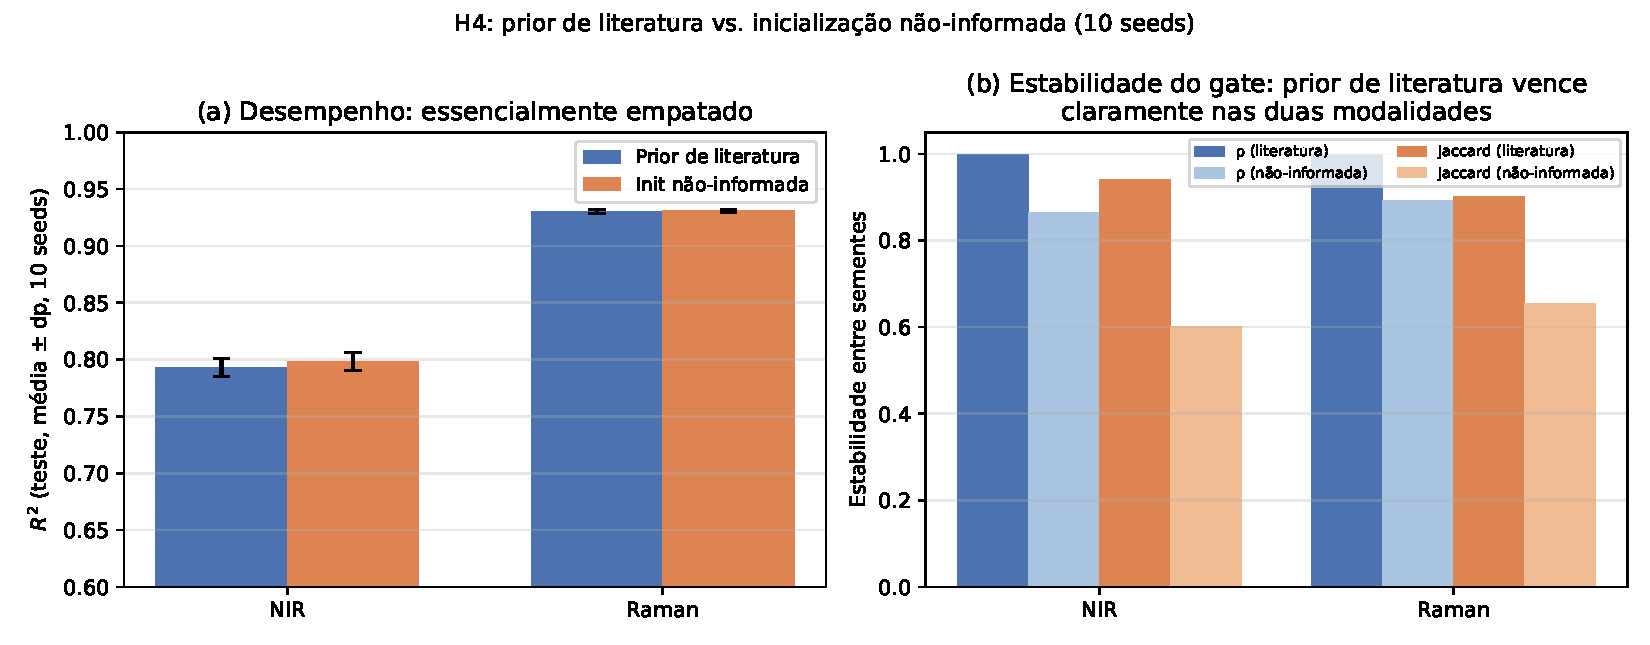
\includegraphics[width=\linewidth]{h4_prior_ablation.pdf}
    \caption{H4: prior de literatura vs.\ inicialização não-informada, 10 sementes, NIR e Raman. (a) Desempenho preditivo ($R^2$ de teste): estatisticamente equivalente nas duas condições. (b) Estabilidade do gate entre sementes ($\rho$ de Pearson e índice de Jaccard, pares de sementes): o prior de literatura produz gates muito mais reprodutíveis entre execuções independentes.}
    \label{fig:h4}
\end{figure}

\paragraph{Interpretação.} O resultado indica que o valor do prior de literatura não está em melhorar a acurácia --- o \texttt{PGSGv2Model} converge para um desempenho preditivo equivalente independentemente da inicialização --- mas em ancorar o gate a uma solução \emph{reprodutível e interpretável}. Sem essa ancoragem, o gate ainda aprende a prever bem, mas a atribuição de importância a bandas específicas varia consideravelmente entre sementes, comprometendo a confiabilidade de qualquer interpretação baseada num único treinamento. Esse padrão se replica em ambas as modalidades, sugerindo que a função do prior --- estabilizar a solução do gate, não necessariamente melhorá-la --- é uma propriedade geral do mecanismo PGSGv2, não específica de NIR.

